\documentclass{standalone}
\usepackage{tikz}
\usetikzlibrary{patterns, positioning}


\begin{document}
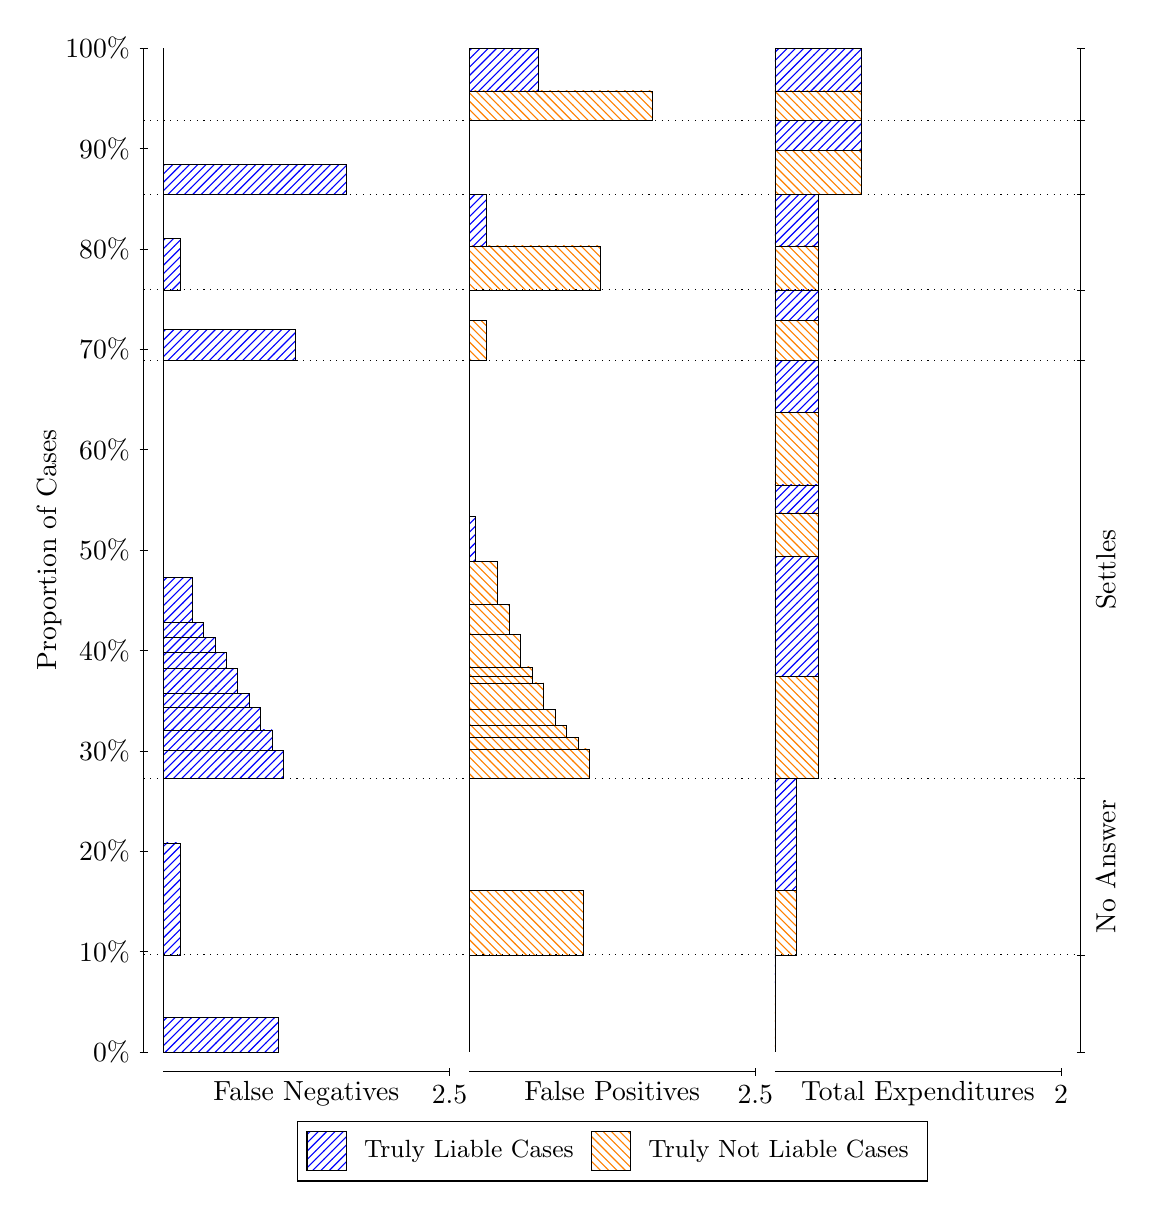
\begin{tikzpicture}
\draw[black, very thin] (1.5,1.75) -- (1.5,14.5);
\node[rotate=90, text=black, anchor=center] at (0.3, 8.125) {Proportion of Cases};
\draw[black, very thin] (1.45,1.75) -- (1.55,1.75);
\node[text=black, anchor=east] at (1.45, 1.75) {0\%};
\draw[black, very thin] (1.45,3.025) -- (1.55,3.025);
\node[text=black, anchor=east] at (1.45, 3.025) {10\%};
\draw[black, very thin] (1.45,4.3) -- (1.55,4.3);
\node[text=black, anchor=east] at (1.45, 4.3) {20\%};
\draw[black, very thin] (1.45,5.575) -- (1.55,5.575);
\node[text=black, anchor=east] at (1.45, 5.575) {30\%};
\draw[black, very thin] (1.45,6.85) -- (1.55,6.85);
\node[text=black, anchor=east] at (1.45, 6.85) {40\%};
\draw[black, very thin] (1.45,8.125) -- (1.55,8.125);
\node[text=black, anchor=east] at (1.45, 8.125) {50\%};
\draw[black, very thin] (1.45,9.4) -- (1.55,9.4);
\node[text=black, anchor=east] at (1.45, 9.4) {60\%};
\draw[black, very thin] (1.45,10.675) -- (1.55,10.675);
\node[text=black, anchor=east] at (1.45, 10.675) {70\%};
\draw[black, very thin] (1.45,11.95) -- (1.55,11.95);
\node[text=black, anchor=east] at (1.45, 11.95) {80\%};
\draw[black, very thin] (1.45,13.225) -- (1.55,13.225);
\node[text=black, anchor=east] at (1.45, 13.225) {90\%};
\draw[black, very thin] (1.45,14.5) -- (1.55,14.5);
\node[text=black, anchor=east] at (1.45, 14.5) {100\%};

\draw[black, very thin] (13.4,1.75) -- (13.4,14.5);
\draw[black, very thin] (13.35,1.75) -- (13.45,1.75);
\node[anchor=west] at (13.35, 1.75) {};
\draw[black, very thin] (13.35,2.9828) -- (13.45,2.9828);
\node[anchor=west] at (13.35, 2.9828) {};
\draw[black, very thin] (13.35,5.2231) -- (13.45,5.2231);
\node[anchor=west] at (13.35, 5.2231) {};
\draw[black, very thin] (13.35,10.534) -- (13.45,10.534);
\node[anchor=west] at (13.35, 10.534) {};
\draw[black, very thin] (13.35,11.429) -- (13.45,11.429);
\node[anchor=west] at (13.35, 11.429) {};
\draw[black, very thin] (13.35,12.639) -- (13.45,12.639);
\node[anchor=west] at (13.35, 12.639) {};
\draw[black, very thin] (13.35,13.584) -- (13.45,13.584);
\node[anchor=west] at (13.35, 13.584) {};
\draw[black, very thin] (13.35,14.5) -- (13.45,14.5);
\node[anchor=west] at (13.35, 14.5) {};

\draw[black, very thin, pattern color=blue, pattern=north east lines] (1.75,1.75) rectangle (3.2033,2.1845);
\draw[black, very thin, pattern color=orange, pattern=north west lines] (1.75,2.1845) rectangle (1.75,2.9828);
\draw[black, very thin, pattern color=blue, pattern=north east lines] (1.75,2.9828) rectangle (1.968,4.4056);
\draw[black, very thin, pattern color=orange, pattern=north west lines] (1.75,4.4056) rectangle (1.75,5.2231);
\draw[black, very thin, pattern color=blue, pattern=north east lines] (1.75,5.2231) rectangle (3.276,5.5791);
\draw[black, very thin, pattern color=blue, pattern=north east lines] (1.75,5.5791) rectangle (3.1307,5.8412);
\draw[black, very thin, pattern color=blue, pattern=north east lines] (1.75,5.8412) rectangle (2.9853,6.1307);
\draw[black, very thin, pattern color=blue, pattern=north east lines] (1.75,6.1307) rectangle (2.84,6.308);
\draw[black, very thin, pattern color=blue, pattern=north east lines] (1.75,6.308) rectangle (2.6947,6.6239);
\draw[black, very thin, pattern color=blue, pattern=north east lines] (1.75,6.6239) rectangle (2.5493,6.8231);
\draw[black, very thin, pattern color=blue, pattern=north east lines] (1.75,6.8231) rectangle (2.404,7.0118);
\draw[black, very thin, pattern color=blue, pattern=north east lines] (1.75,7.0118) rectangle (2.2587,7.2062);
\draw[black, very thin, pattern color=blue, pattern=north east lines] (1.75,7.2062) rectangle (2.1133,7.7739);
\draw[black, very thin, pattern color=orange, pattern=north west lines] (1.75,7.7739) rectangle (1.75,10.534);
\draw[black, very thin, pattern color=blue, pattern=north east lines] (1.75,10.534) rectangle (3.4213,10.923);
\draw[black, very thin, pattern color=orange, pattern=north west lines] (1.75,10.923) rectangle (1.75,11.429);
\draw[black, very thin, pattern color=blue, pattern=north east lines] (1.75,11.429) rectangle (1.968,12.082);
\draw[black, very thin, pattern color=orange, pattern=north west lines] (1.75,12.082) rectangle (1.75,12.639);
\draw[black, very thin, pattern color=blue, pattern=north east lines] (1.75,12.639) rectangle (4.0753,13.019);
\draw[black, very thin, pattern color=orange, pattern=north west lines] (1.75,13.019) rectangle (1.75,13.584);
\draw[black, very thin, pattern color=orange, pattern=north west lines] (1.75,13.584) rectangle (1.75,13.955);
\draw[black, very thin, pattern color=blue, pattern=north east lines] (1.75,13.955) rectangle (1.75,14.5);
\draw[black, very thin, pattern color=orange, pattern=north west lines] (5.6333,1.75) rectangle (5.6333,2.5483);
\draw[black, very thin, pattern color=blue, pattern=north east lines] (5.6333,2.5483) rectangle (5.6333,2.9828);
\draw[black, very thin, pattern color=orange, pattern=north west lines] (5.6333,2.9828) rectangle (7.0867,3.8002);
\draw[black, very thin, pattern color=blue, pattern=north east lines] (5.6333,3.8002) rectangle (5.6333,5.2231);
\draw[black, very thin, pattern color=orange, pattern=north west lines] (5.6333,5.2231) rectangle (7.1593,5.6004);
\draw[black, very thin, pattern color=orange, pattern=north west lines] (5.6333,5.6004) rectangle (7.014,5.7453);
\draw[black, very thin, pattern color=orange, pattern=north west lines] (5.6333,5.7453) rectangle (6.8687,5.8969);
\draw[black, very thin, pattern color=orange, pattern=north west lines] (5.6333,5.8969) rectangle (6.7233,6.1);
\draw[black, very thin, pattern color=orange, pattern=north west lines] (5.6333,6.1) rectangle (6.578,6.4372);
\draw[black, very thin, pattern color=orange, pattern=north west lines] (5.6333,6.4372) rectangle (6.4327,6.5172);
\draw[black, very thin, pattern color=orange, pattern=north west lines] (5.6333,6.5172) rectangle (6.4327,6.6404);
\draw[black, very thin, pattern color=orange, pattern=north west lines] (5.6333,6.6404) rectangle (6.2873,7.049);
\draw[black, very thin, pattern color=orange, pattern=north west lines] (5.6333,7.049) rectangle (6.142,7.4347);
\draw[black, very thin, pattern color=orange, pattern=north west lines] (5.6333,7.4347) rectangle (5.9967,7.9833);
\draw[black, very thin, pattern color=blue, pattern=north east lines] (5.6333,7.9833) rectangle (5.706,8.5509);
\draw[black, very thin, pattern color=blue, pattern=north east lines] (5.6333,8.5509) rectangle (5.6333,10.534);
\draw[black, very thin, pattern color=orange, pattern=north west lines] (5.6333,10.534) rectangle (5.8513,11.04);
\draw[black, very thin, pattern color=blue, pattern=north east lines] (5.6333,11.04) rectangle (5.6333,11.429);
\draw[black, very thin, pattern color=orange, pattern=north west lines] (5.6333,11.429) rectangle (7.3047,11.986);
\draw[black, very thin, pattern color=blue, pattern=north east lines] (5.6333,11.986) rectangle (5.8513,12.639);
\draw[black, very thin, pattern color=orange, pattern=north west lines] (5.6333,12.639) rectangle (5.6333,13.204);
\draw[black, very thin, pattern color=blue, pattern=north east lines] (5.6333,13.204) rectangle (5.6333,13.584);
\draw[black, very thin, pattern color=orange, pattern=north west lines] (5.6333,13.584) rectangle (7.9587,13.955);
\draw[black, very thin, pattern color=blue, pattern=north east lines] (5.6333,13.955) rectangle (6.5053,14.5);
\draw[black, very thin, pattern color=orange, pattern=north west lines] (9.5167,1.75) rectangle (9.5167,2.5483);
\draw[black, very thin, pattern color=blue, pattern=north east lines] (9.5167,2.5483) rectangle (9.5167,2.9828);
\draw[black, very thin, pattern color=orange, pattern=north west lines] (9.5167,2.9828) rectangle (9.7892,3.8002);
\draw[black, very thin, pattern color=blue, pattern=north east lines] (9.5167,3.8002) rectangle (9.7892,5.2231);
\draw[black, very thin, pattern color=orange, pattern=north west lines] (9.5167,5.2231) rectangle (10.062,6.5172);
\draw[black, very thin, pattern color=blue, pattern=north east lines] (9.5167,6.5172) rectangle (10.062,8.0486);
\draw[black, very thin, pattern color=orange, pattern=north west lines] (9.5167,8.0486) rectangle (10.062,8.5972);
\draw[black, very thin, pattern color=blue, pattern=north east lines] (9.5167,8.5972) rectangle (10.062,8.9532);
\draw[black, very thin, pattern color=orange, pattern=north west lines] (9.5167,8.9532) rectangle (10.062,9.8707);
\draw[black, very thin, pattern color=blue, pattern=north east lines] (9.5167,9.8707) rectangle (10.062,10.534);
\draw[black, very thin, pattern color=orange, pattern=north west lines] (9.5167,10.534) rectangle (10.062,11.04);
\draw[black, very thin, pattern color=blue, pattern=north east lines] (9.5167,11.04) rectangle (10.062,11.429);
\draw[black, very thin, pattern color=orange, pattern=north west lines] (9.5167,11.429) rectangle (10.062,11.986);
\draw[black, very thin, pattern color=blue, pattern=north east lines] (9.5167,11.986) rectangle (10.062,12.639);
\draw[black, very thin, pattern color=orange, pattern=north west lines] (9.5167,12.639) rectangle (10.607,13.204);
\draw[black, very thin, pattern color=blue, pattern=north east lines] (9.5167,13.204) rectangle (10.607,13.584);
\draw[black, very thin, pattern color=orange, pattern=north west lines] (9.5167,13.584) rectangle (10.607,13.955);
\draw[black, very thin, pattern color=blue, pattern=north east lines] (9.5167,13.955) rectangle (10.607,14.5);
\draw[black, dotted] (1.5,2.9828) -- (13.4,2.9828);
\draw[black, dotted] (1.5,5.2231) -- (13.4,5.2231);
\draw[black, dotted] (1.5,10.534) -- (13.4,10.534);
\draw[black, dotted] (1.5,11.429) -- (13.4,11.429);
\draw[black, dotted] (1.5,12.639) -- (13.4,12.639);
\draw[black, dotted] (1.5,13.584) -- (13.4,13.584);
\draw[black, very thin] (1.75,1.5) -- (5.3833,1.5);
\node[text=black, anchor=north] at (3.5667, 1.5) {False Negatives};
\draw[black, very thin] (5.3833,1.45) -- (5.3833,1.55);
\node[text=black, anchor=north] at (5.3833, 1.45) {2.5};

\draw[black, very thin] (5.6333,1.5) -- (9.2667,1.5);
\node[text=black, anchor=north] at (7.45, 1.5) {False Positives};
\draw[black, very thin] (9.2667,1.45) -- (9.2667,1.55);
\node[text=black, anchor=north] at (9.2667, 1.45) {2.5};

\draw[black, very thin] (9.5167,1.5) -- (13.15,1.5);
\node[text=black, anchor=north] at (11.333, 1.5) {Total Expenditures};
\draw[black, very thin] (13.15,1.45) -- (13.15,1.55);
\node[text=black, anchor=north] at (13.15, 1.45) {2};


\node[text=black, centered, rotate=90] at (13.72, 4.1029) {No Answer};
\node[text=black, centered, rotate=90] at (13.72, 7.8786) {Settles};





\draw (7.449999999999999,1.5) node[draw=none] (baseCoordinate) {};
\begin{scope}[align=center]
        \matrix[scale=0.5, draw=black, below=0.5cm of baseCoordinate, nodes={draw}, column sep=0.1cm]{
            \node[rectangle, draw, minimum width=0.5cm, minimum height=0.5cm, pattern color=blue, pattern=north east lines] {}; &
            \node[draw=none, font=\small, text=black] (B) {Truly Liable Cases}; &
            \node[rectangle, draw, minimum width=0.5cm, minimum height=0.5cm, pattern color=orange, pattern=north west lines] {}; &
            \node[draw=none, font=\small, text=black] (B) {Truly Not Liable Cases}; \\
            };
\end{scope}

\end{tikzpicture}
\end{document}